\documentclass{beamer}
\usepackage{graphicx}
\usepackage{epstopdf}

\title{$P$-Wave Charmonia Production in Exclusive $B_c$-Meson Decays}
\author{Alexey Luchinsky}

\newcommand{\R}{\mathcal{R}}
\newcommand{\M}{\mathcal{M}}
\newcommand{\A}{\mathcal{A}}


\begin{document}

\begin{frame}
  \maketitle
\end{frame}

\begin{frame}
  \frametitle{Content}
  \tableofcontents
\end{frame}

\section{Introduction}
\begin{frame}
  \frametitle{Introduction}
\end{frame}

\section{$B_c\to J/\psi + \R$}

\subsection{General Info}

\begin{frame}[t]
  \frametitle{$B_c\to J/\psi+\R$}
  Diagram and amplitude factorise:
  \begin{center}
    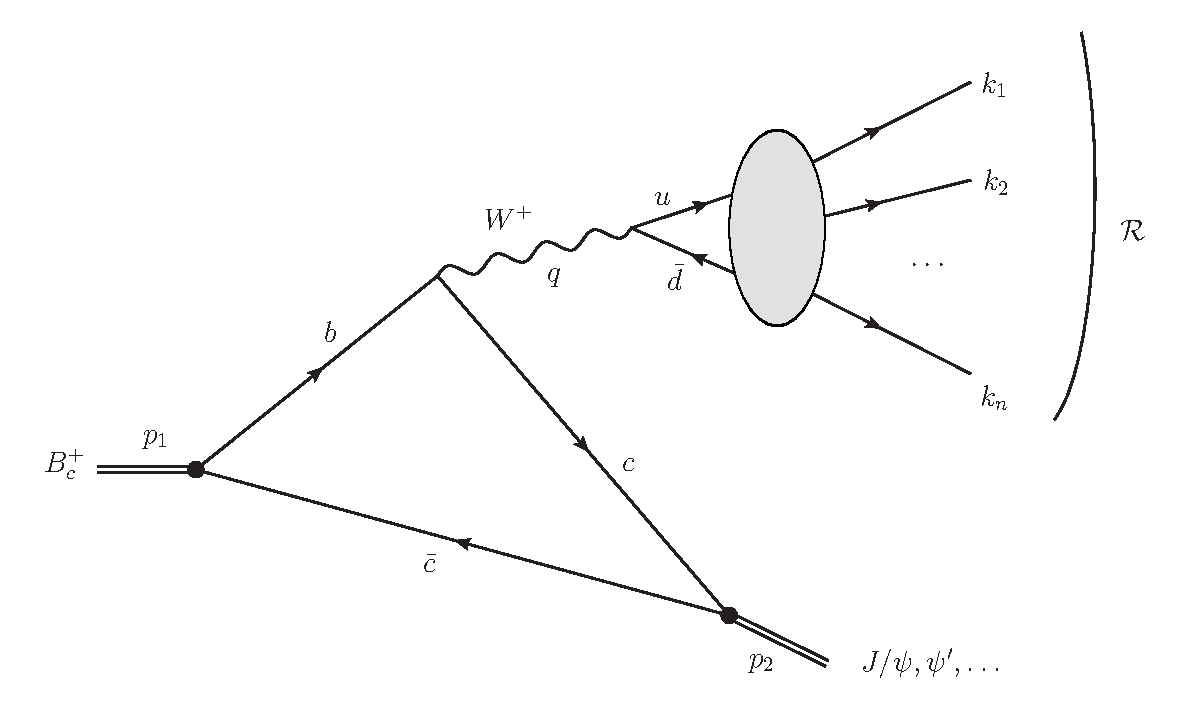
\includegraphics[width=0.5\columnwidth]{figs/diags_BcCCW}
  \end{center}
      $$\M\left(B_c \to J/\psi + \R\right) = H^\mu \epsilon^{(\R)}_\mu$$
   where
   \begin{itemize}
   \item $H^\mu$ is the $B_c\to J/\psi W$ transition vertex
   \item $\epsilon^{(\R)}_\mu$ is effective  $W\to\R$ polarization vector
   \end{itemize}
The differential width is
$$
\frac{d\Gamma}{dq^2} \sim \frac{d\Gamma_T}{dq^2} \rho_T\left(q^2\right) + \frac{d\Gamma_L}{dq^2} \rho_L\left(q^2\right)
$$
\end{frame}


\begin{frame}
  \frametitle{$B_c \to J/\psi W$ transition}
\end{frame}

\begin{frame}
  \frametitle{$W\to R$ polarization vector}
\end{frame}

\subsection{$B_c\to J/\psi e\nu$}
\begin{frame}
  \frametitle{$B_c\to J/\psi e\nu$}
\end{frame}

\subsection{$B_c\to J/\psi \pi$, $B_c\to J/\psi \rho$}
\begin{frame}
  \frametitle{$B_c\to J/\psi \pi$, $B_c\to J/\psi \rho$}
\end{frame}

\subsection{$B_c\to J/\psi + n\pi$}
\begin{frame}
  \frametitle{$B_c\to J/\psi+ 2\pi$}
\end{frame}

\begin{frame}
  \frametitle{$B_c\to J/\psi + 3\pi$}
\end{frame}

\begin{frame}
  \frametitle{$B_c\to J/\psi +  5\pi$}
\end{frame}


\section{$B_c\to \chi_{cJ}+\R$}
\begin{frame}
  \frametitle{$B_c\to \chi_{cJ}+\R$}
\begin{center}
  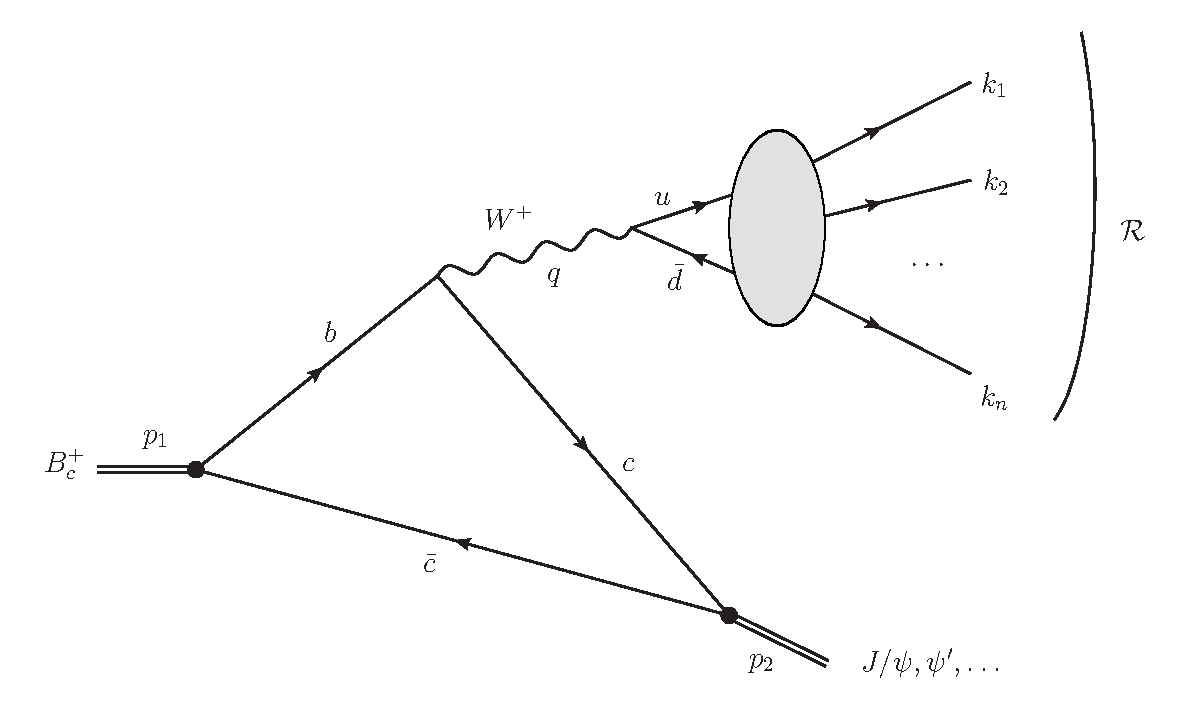
\includegraphics[width=0.5\columnwidth]{figs/diags_BcCCW}
\end{center}
$$\M\left(B_c \to chi_{cJ} + \R\right) = H^\mu \epsilon^{(\R)}_\mu$$
Form-factors of the $B_c\to \chi_{cJ}W$ transitions were considered in
\begin{itemize}
\item Ebert
\item Wang
\item Hernandez
\item etc.
\end{itemize}
\end{frame}

\subsection{$\chi_{c0}$}
\begin{frame}
  \frametitle{$\chi_{c0}$}
  $$
  H_\mu = f_{+}\left(q^2\right) \left(p_1+p_2\right)_\mu + f_{-}\left(q^2\right) \left(p_1-p_2\right)_\mu 
  $$
  
\end{frame}


\subsection{$\chi_{c1}$}
\begin{frame}
  \frametitle{$\chi_{c1}$}
\end{frame}

\subsection{$\chi_{c2}$}
\begin{frame}
  \frametitle{$\chi_{c2}$}
\end{frame}



  
\section{$B_c\to \chi_{cJ}+n\pi$}
\begin{frame}
  \frametitle{$B_c\to \chi_{cJ}+n\pi$}
\end{frame}

\section{EvtGen}
\begin{frame}
  \frametitle{EvtGen}
\end{frame}


\section{Conclusion}
\begin{frame}
  \frametitle{Conclusion}
\end{frame}


\end{document}
